% ======================================================================
%  Replacement for the Figure 2 (drag-to-edit) block.
%  New, generality-oriented edit figure: 2 scenes x 2 drag directions,
%  with control-node handle outline, applied-drag arrow, and a per-pixel
%  edit-magnitude heatmap + shared colorbar.
%
%  Uses only graphicx (\rotatebox, \includegraphics) -- already loaded by
%  the Wiley class. New image files (nothing existing is overwritten):
%    figures/edit_gen_pulling_{before,down,right,diff}.png
%    figures/edit_gen_cutting_{before,down,left,diff}.png
%    figures/edit_gen_colorbar.png
%  Alternate direction panels are also available if you want to swap one:
%    figures/edit_gen_pulling_up.png , figures/edit_gen_cutting_right.png
% ======================================================================
\begin{figure*}[t]
\centering
\footnotesize
\setlength{\tabcolsep}{1.2pt}
\renewcommand{\arraystretch}{0.4}
\begin{minipage}{0.93\textwidth}
\begin{tabular}{@{}ccccc@{}}
 & before & drag $\downarrow$ & lateral drag & edit magnitude \\[1pt]
\rotatebox{90}{\hspace{4pt}\texttt{pulling}} &
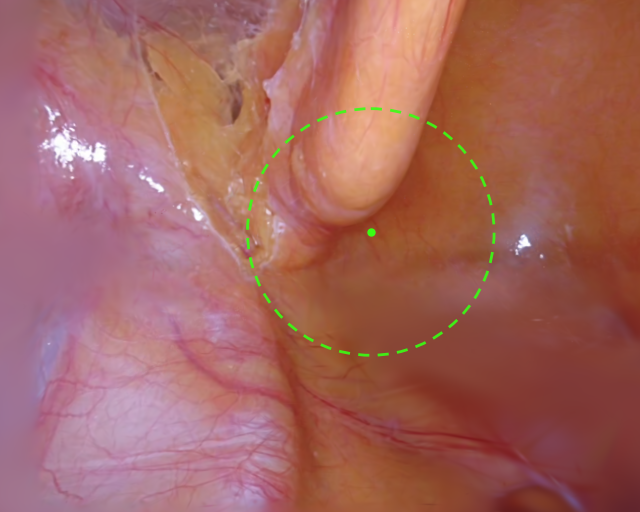
\includegraphics[width=0.225\textwidth]{figures/edit_gen_pulling_before.png} &
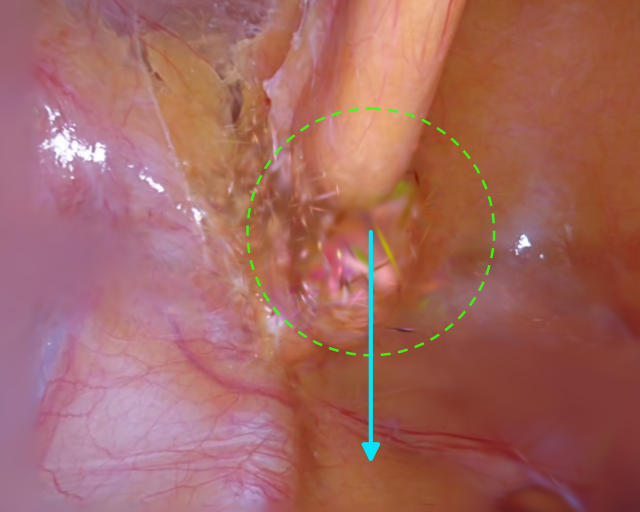
\includegraphics[width=0.225\textwidth]{figures/edit_gen_pulling_down.png} &
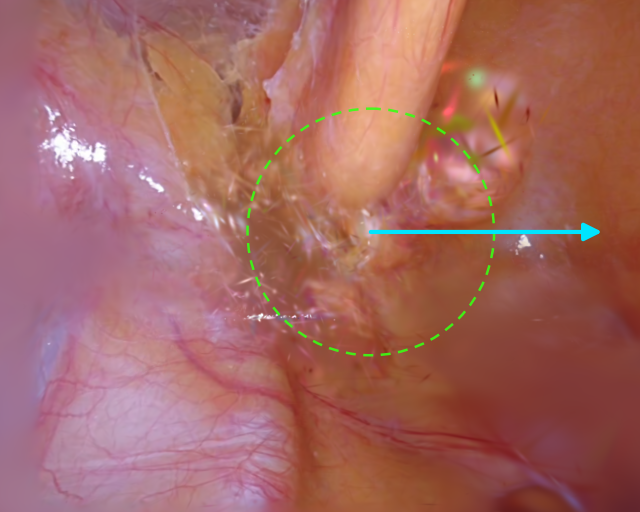
\includegraphics[width=0.225\textwidth]{figures/edit_gen_pulling_right.png} &
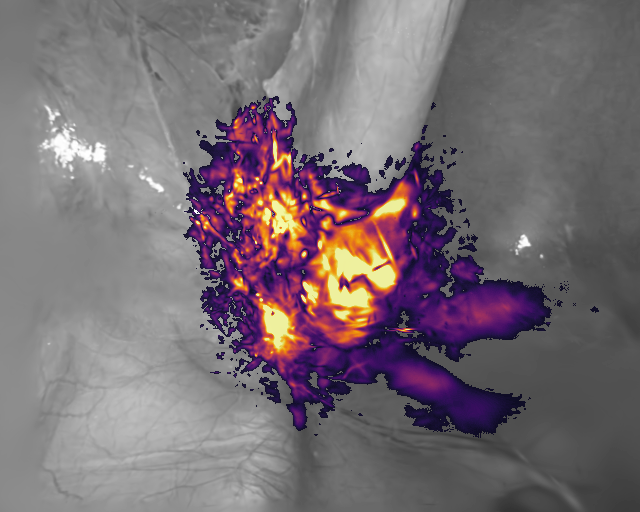
\includegraphics[width=0.225\textwidth]{figures/edit_gen_pulling_diff.png} \\[1pt]
\rotatebox{90}{\hspace{4pt}\texttt{cutting}} &
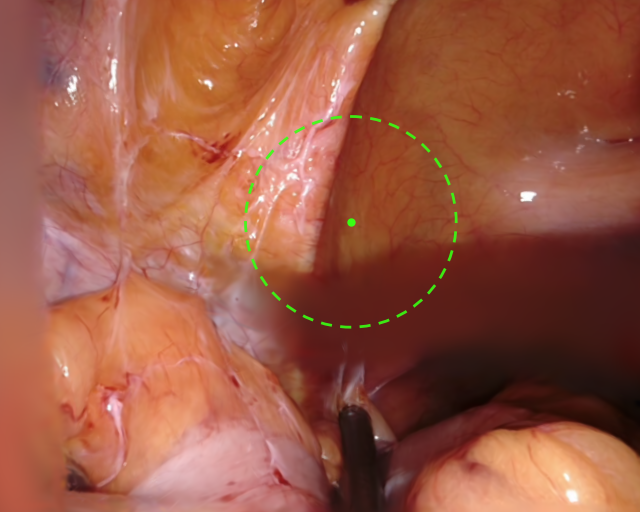
\includegraphics[width=0.225\textwidth]{figures/edit_gen_cutting_before.png} &
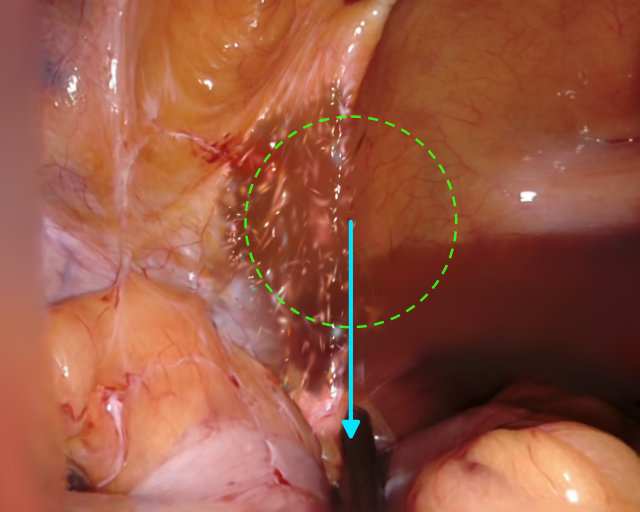
\includegraphics[width=0.225\textwidth]{figures/edit_gen_cutting_down.png} &
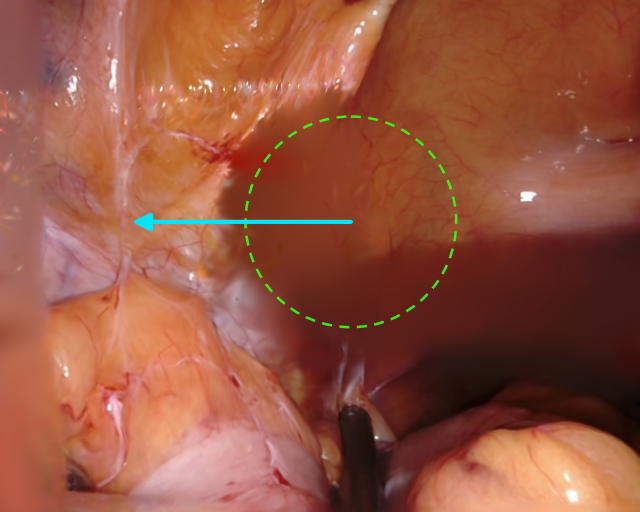
\includegraphics[width=0.225\textwidth]{figures/edit_gen_cutting_left.png} &
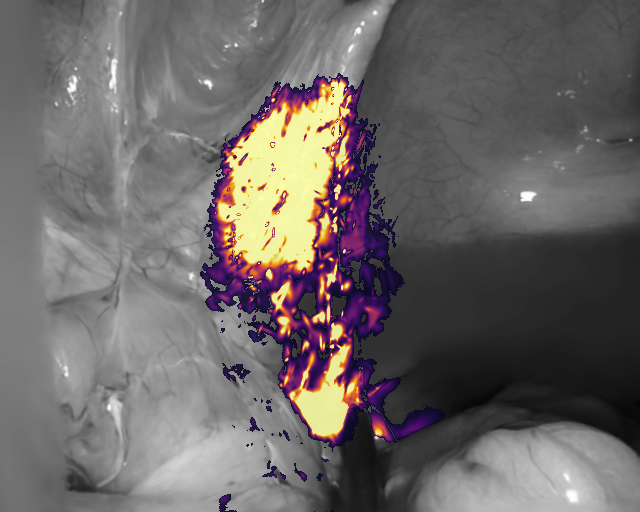
\includegraphics[width=0.225\textwidth]{figures/edit_gen_cutting_diff.png} \\
\end{tabular}
\end{minipage}\hfill
\begin{minipage}{0.055\textwidth}
\centering
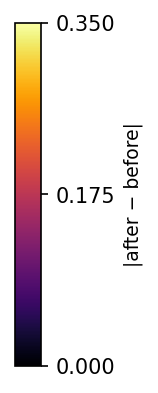
\includegraphics[height=95pt]{figures/edit_gen_colorbar.png}
\end{minipage}
\caption{Qualitative drag-to-edit generality. Each row is a scene
(\texttt{pulling\_soft\_tissues}, \texttt{cutting\_tissues\_twice}); each edit applies
an inference-time translation to a local group of control nodes and re-renders the
same view without retraining. The dashed outline marks the grabbed control-node
region and the cyan arrow shows the applied node translation. Columns 2--3 drag the
same handle in different directions (vertical and lateral). The last column is the
per-pixel edit magnitude $\lVert I_{\mathrm{after}}-I_{\mathrm{before}}\rVert$, which
stays localized to the manipulated region. The examples illustrate the locality and
directional controllability of the weighted node operation; they do not establish
biomechanical validity.\label{fig:edit}}
\end{figure*}
